\section{Projekty v\'yskumnej skupiny MONICA}

\subsection{Meracia platforma BasicMeter}

BasicMeter \citep{monica} je jedným z projektov výskumnej 
skupiny MONICA, sídliacej v Laboratóriu počítačových sietí (CNL) na Technickej Univerzite v Košiciach. 
Je to merací nástroj založený na protokole IPFIX. Slúži na pasívne meranie parametrov prevádzky 
počítačových sietí a ich následné vyhodnocovanie. Začiatky vývoja siahajú až do roku 2003. Jeho 
architektúra je znázornená na Obrázku \ref{o:bm_architecture}.

\begin{figure}[ht!]
\centering
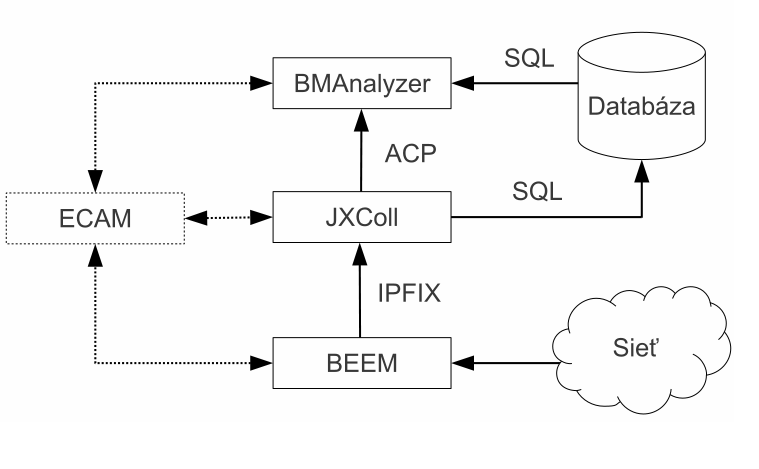
\includegraphics[width=0.7\textwidth]{bm_architecture}
\caption{Architektúra nástroja BasicMeter \citep{ja}}\label{o:bm_architecture}
\end{figure}

Platforma pozostáva z nasledujúcich komponentov:
\begin{itemize}
 \item \textbf{BEEM} - merací a exportovací proces - exportér
 \item \textbf{JXColl} - zhromažďovací proces - kolektor
 \item \textbf{BMAnalyzer} - aplikácia na vyhodnocovanie údajov
 \item \textbf{ECAM} - riadiaci komponent nástroja
 \item \textbf{bmIDS} - systém pre detekciu narušenia
\end{itemize}

Najnižšou vrstvou architektúry je \emph{BEEM}. Zabezpečuje všetky funkcie 
meracieho a exportovacieho procesu definovaného v špecifikácii IPFIX. Namerané záznamy o tokoch
posiela komponentu \emph{JXColl} vo formáte IPFIX správ. Kolektor dekóduje prijaté správy od jedného
alebo viacerých exportérov a ukladá ich do databázy kvôli neskoršej analýze. Za účelom analyzovania dát
a ich grafického zobrazenia vo forme grafov v reálnom čase ich posiela komponentu \emph{BMAnalyzer} 
prostredníctvom 
protokolu ACP \citep{ado}. \emph{bmIDS} tak isto prijíma dáta v reálnom čase, no jeho úlohou je analyzovať
prebiehajúcu komunikáciu v uzli siete a odhaľovať pripadné útoky, resp. anomálie. \emph{ECAM} umožňuje 
centrálne riadiť beh jednotlivých častí architektúry. Medzi jeho funkcie patrí vytvorenie a zmazanie 
inštancie exportérov a kolektorov, prípadne meniť ich konfiguráciu. \citep{ja, veri}

\subsection{Merací nástroj SLAmeter}

SLAmeter je merač parametrov sieťovej prevádzky vyhodnocujúci dodržiavanie zmluvy o úrovni poskytovanej 
služby \emph{(SLA)}. V tomto prípade sa pod poskytovanou službou rozumie prístup do siete 
Internet. Základ nástroja je postavený na komponentoch nástroja BasicMeter, a rovnako je projektom 
výskumnej skupiny MONICA. 

Cieľom nástroja je spracovať vybrané parametre sieťovej prevádzky a vypočítať z nich akúsi triedu 
kvality. SLAmeter slúži každému, kto si chce skontrolovať kvalitu svojho pripojenia do Internetu. 
Triedy umožňujú jednoduchý spôsob porovnávania jednotlivých pripojení ponúkané poskytovateľmi, 
čo by malo mať dopad na konkurenčný boj a zvýšenie snahy o zlepšovanie kvality služieb. \citep{slameter}

Ako bolo spomenuté, SLAmeter je akousi nadstavbou na BasicMeter. Jeho architektúra pozostáva z exportérov,
ktoré posielajú namerané záznamy o tokoch zhromažďovaču. Ten spracováva záznamy a ukladá ich do 
centrálnej databázy. Úlohou \emph{Vyhodnocovača} je na základe požiadaviek od webového rozhrania 
spracovávať IPFIX záznamy a vytvárať tak štatistické a analytické údaje o charaktere 
meranej sieťovej prevádzky \citep{evaluator}. \emph{Webové rozhranie} je modulárna webová aplikácia 
s pohľadmi pre zákazníka a poskytovateľa Internetových služieb.

Príklad architektúry nástroja SLAmeter so zapojením Mediátora je na Obrázku \ref{o:sla_architecture}.
BEEM môže exportovať IPFIX správy priamo kolektoru JXColl. No v prípade, že chce využiť sprostredkovateľské 
procesy na modifikáciu údajov, posiela správy Mediátoru a ten ich ďalej preposiela kolektoru.

\begin{figure}[ht!]
\centering
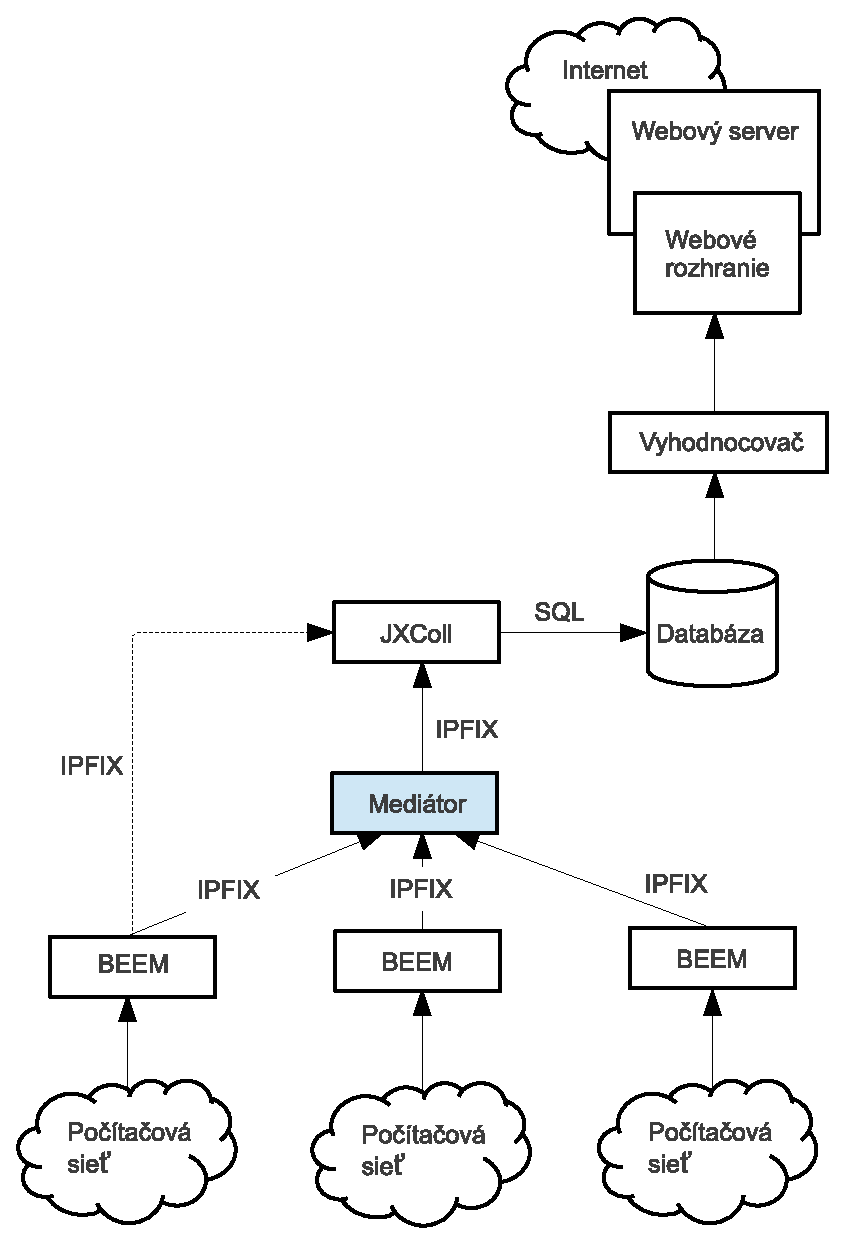
\includegraphics[width=0.7\textwidth]{sla_architecture}
\caption{Príklad architektúry nástroja SLAmeter s využitím Mediátora}\label{o:sla_architecture}
\end{figure}